\documentclass{article}
\usepackage{amsmath, amssymb}
\usepackage{MnSymbol}
\usepackage{wasysym}
\usepackage[toc,page]{appendix}
\usepackage{hyperref}
\usepackage{graphicx}
\usepackage{float}
\usepackage[numbered,framed]{matlab-prettifier}
\usepackage[export]{adjustbox}
\begin{document}
	\begin{center}
		\LARGE \bfseries{Answers to Problem Set 4}\\
		Group name: Ferienspass\vspace{.5cm}\\
		\normalsize \normalfont
		Sebastian K\"uhnl: 5642348\\
		Alexander D\"uck (as: reebyte): 5504077\\
		Patrick Blank (as: paddyblank): 6729110\\
		Christian Wierschem: 6729288
	\end{center}
	\normalsize	
	\section{Question 1}
	Chebyshev approximation using equidistant nodes and Chebyshev nodes. However, there is a difference between lecture slides 7 and the notes from the lecture, as you will see in the code provided below.
	Plots are ordered in chronological order! (For comparison, the residuals to actual function are plotted.)\\
	\begin{figure}[h]
	  \begin{minipage}{0.56\textwidth}
	  	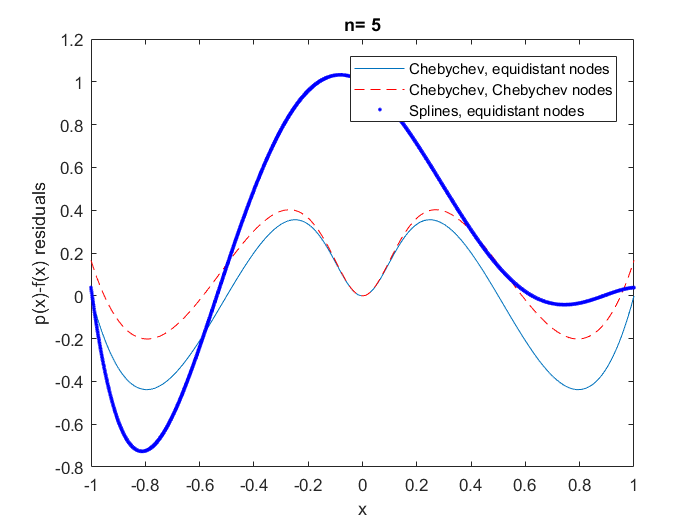
\includegraphics[width = \textwidth, keepaspectratio]{n5res.png}
	  \end{minipage}
	  \begin{minipage}{0.56\textwidth}
	    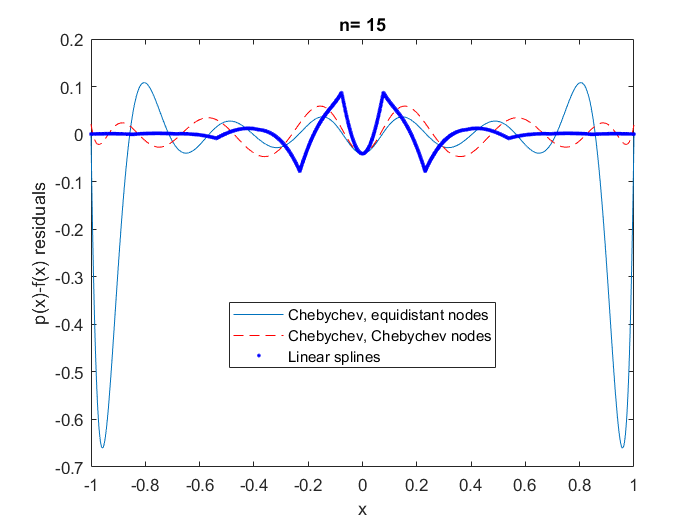
\includegraphics[width = \textwidth, keepaspectratio]{n15res.png}
      \end{minipage}
   	  \begin{minipage}{0.56\textwidth}
   	  	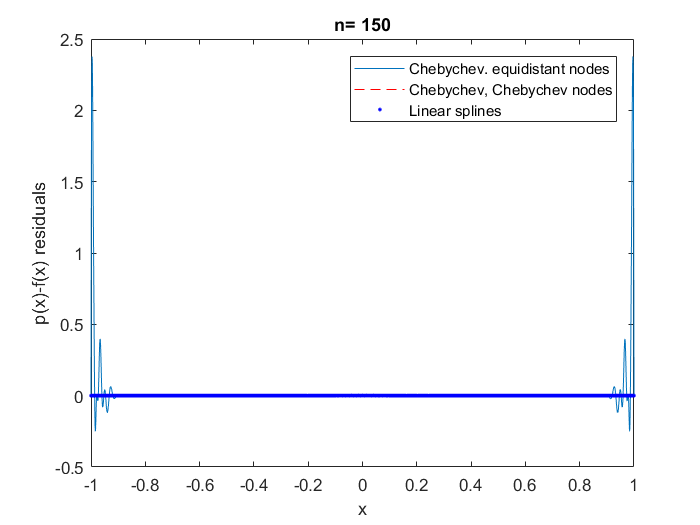
\includegraphics[width = \textwidth, keepaspectratio]{n150res.png}
   	  \end{minipage}   	   
    \end{figure}\\
   For n=5, equidistant nodes and Chebyshev nodes as well as linear splines are very similar. For n=15, linear splines become more edgy. It performs well at the edges and average else. Both Chebyshev approximations are very similar in [-0.75;0.75], while equidistant nodes fall off at the edges (as expected). For n=150 this effect is even stronger, but it moves closer to the corner. The others are not comparable due to the residual scale. The effect does not occur when using Chebyshev nodes because there are more nodes at the corner to prevent these large fluctuations.\\
	\begin{figure}[h]
	\begin{minipage}{0.56\textwidth}
	  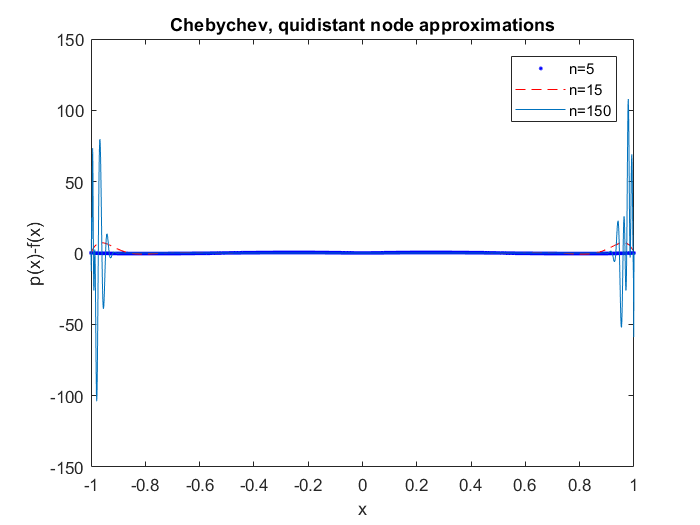
\includegraphics[width = \textwidth, keepaspectratio]{chebequi.png}
    \end{minipage}
    \begin{minipage}{0.56\textwidth}
	  \includegraphics[width = \textwidth, keepaspectratio]{chebcheb.png}
    \end{minipage}
    \begin{minipage}{0.56\textwidth}
	  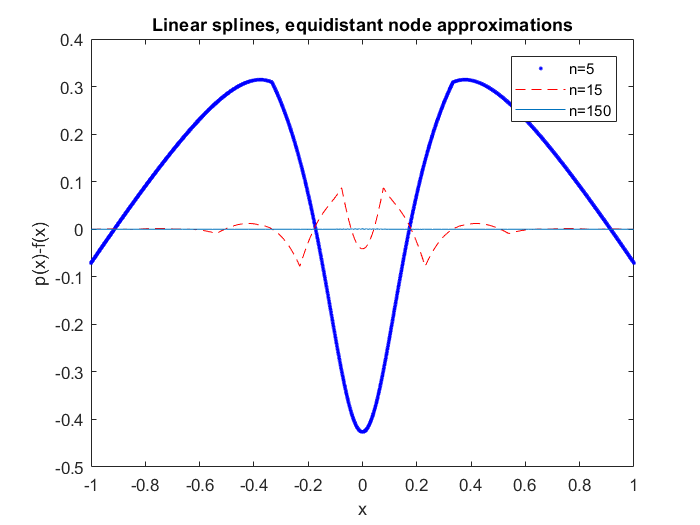
\includegraphics[width = \textwidth, keepaspectratio]{splequi.png}
    \end{minipage}   	   
    \end{figure}\\
    In this figure again the effect of equidistant nodes when using Chebyshev can be seen as large fluctuations at the corner. Besides this, as the number of nodes increases, the approximation gets closer to the real function.\\
    \newpage
	\begin{figure}[h]
	\begin{minipage}{0.56\textwidth}
	  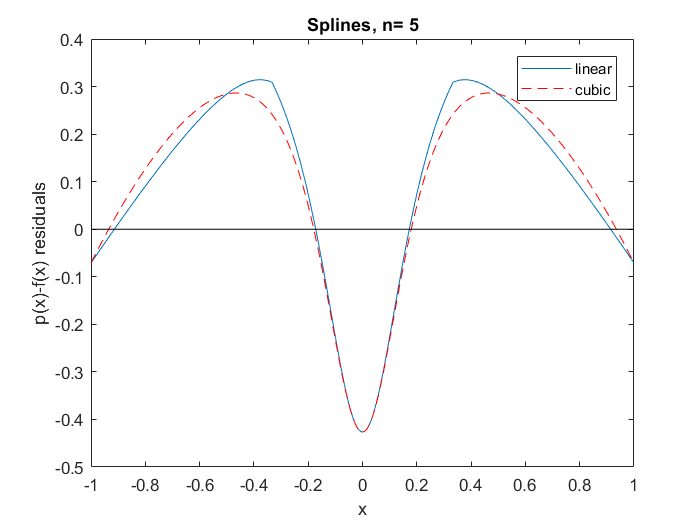
\includegraphics[width = \textwidth, keepaspectratio]{n5lincub.png}
    \end{minipage}
    \begin{minipage}{0.56\textwidth}
	  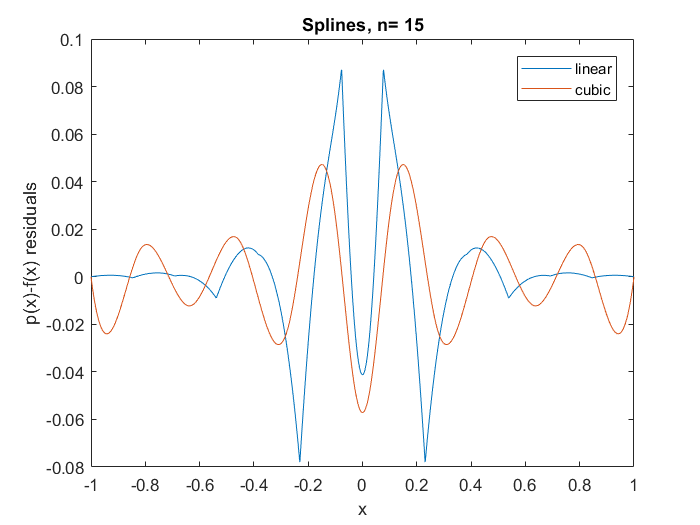
\includegraphics[width = \textwidth, keepaspectratio]{n15lincub.png}
    \end{minipage}
    \begin{minipage}{0.56\textwidth}
	  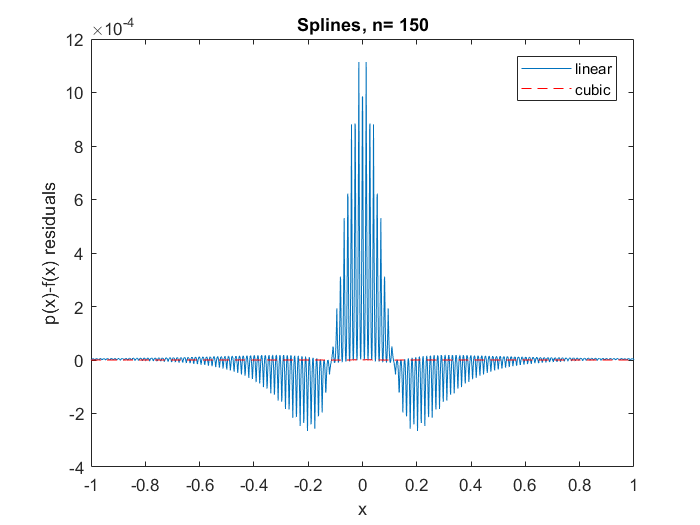
\includegraphics[width = \textwidth, keepaspectratio]{n150lincub.png}
    \end{minipage}   	   
    \end{figure}
    Linear and cubic splines are very similar when n=5. For n=15 one can observe that cubic splines are smoother than linear splines and perform better in the center (around 0), whereas linear splines perform better at the corner (it becomes smooth and then becomes nearly a straight line). For n=150, at first sight, linear splines perform badly, but it is only relative to cubic splines (look at the scale). As n increases, the approximation gets better when using splines.\\
    \newpage
	\begin{figure}[h]
	\begin{minipage}{0.56\textwidth}
	  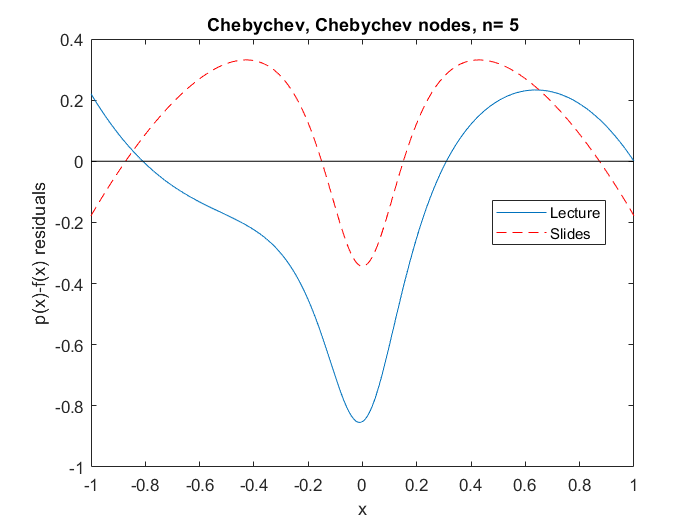
\includegraphics[width = \textwidth, keepaspectratio]{n5lecsli.png}
    \end{minipage}
    \begin{minipage}{0.56\textwidth}
	  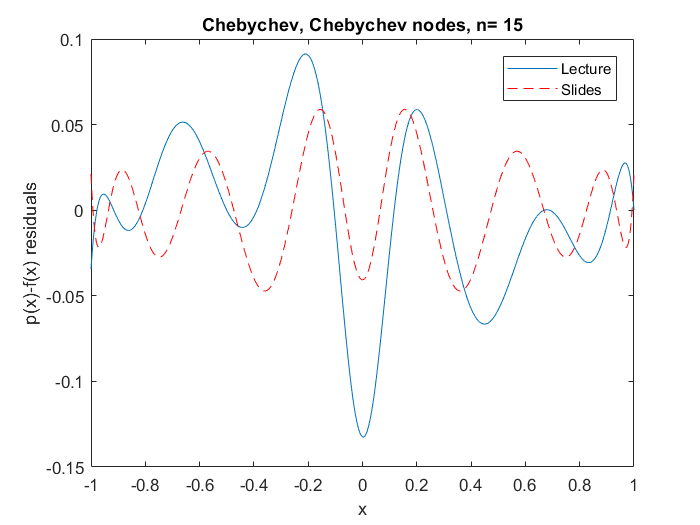
\includegraphics[width = \textwidth, keepaspectratio]{n15lecsli.png}
    \end{minipage}
    \begin{minipage}{0.56\textwidth}
	  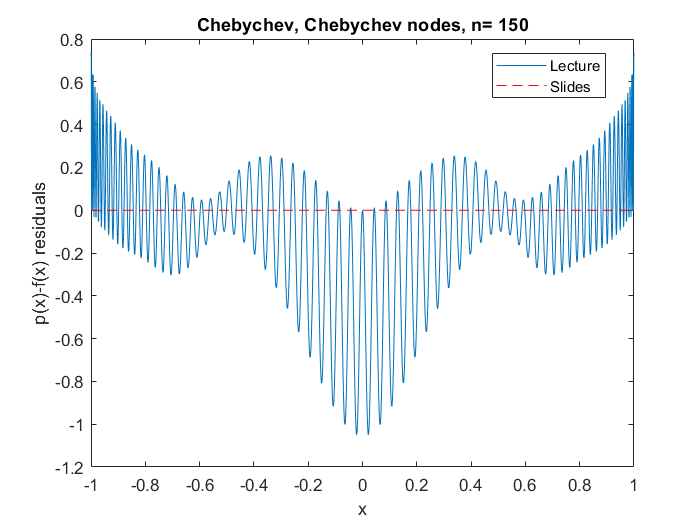
\includegraphics[width = \textwidth, keepaspectratio]{n150lecsli.png}
    \end{minipage}   	   
    \end{figure}
    The slides formula seems to be the right one. The function is symmetric and so is the approximation. The lecture formula leads to very odd (i.e. asymmetric) approximations.\\\\
    In general, it seems to be very odd that the residuals at 0 are not 0, because there should be a node and thus the residual should be zero. Maybe it is due to the toolbox calculations. Other possibilities have been thought of and precluded.
\newpage

\section{Question 2}
The first order condition of the unconstrained maximisation problem is given by
\begin{equation*}
u^\prime(C_0) - \mathbb{E}u^\prime(W_0 (1+r) - C_0) = 0
\end{equation*}
Accordingly, the optimal consumption plan obeys the Euler equation
\begin{equation}
u^\prime(C_0) = \mathbb{E}u^\prime(C_1) \tag{Euler EQ}
\end{equation}

\paragraph{Quadratic utility}
Let the utility function be quadratic. Then, marginal utility is given by
\begin{align*}
u^\prime(C_t) &= -(C_t - \bar{C}) = \bar{C} - C_t \tag{Marginal utility}\\
\intertext{Moreover,}
u^{\prime\prime}(C_t) &= -1 < 0 \tag{Risk aversion}\\
u^{\prime\prime\prime}(C_t) &= 0 \tag{Prudence}
\end{align*}
In order to obtain the optimal consumption, plug the marginal utility into the Euler equation
\begin{align*}
\bar{C} - C_0 &= \mathbb{E}(\bar{C} - C_1) \notag \\
\bar{C} - C_0 &= \mathbb{E}(\bar{C} - (W_0 (1+r) - C_0)) \notag \\
2 C_0 &= W_0 \mathbb{E}(1+r) \notag \\
C_0 &= \frac{1}{2} W_0 \mathbb{E}(1+r) \notag
\end{align*}
Note that marginal utility is linear in $C_t$. Consequently, we could exploit linearity of the expectation operator which yields more generally
\begin{equation*}
\mathbb{E}(u^\prime(C_t)) = u^\prime(\mathbb{E}(C_t))
\end{equation*}
This is why certainty equivalence holds, i.e., the intertemporal consumption decision remains unchanged when agents are exposed to more or even less uncertainty. Indeed, expected lifetime utility is reduced by income risks (concave utility). However, the comparative statics require to look at the third derivative which indicates that agents are not influenced by the degree of income uncertainty. In case of linear marginal utility agents are not prudent. It is quite hard to judge whether this result makes economic sense, i.e., such a function provides a meaningful utility representation. There is a lot of empirical work on the willingness to insure, it is true, but prudence is a different issue. If we believe in the precautionary savings motive (which makes intuitively sense), quadratic utility is inappropriate.

\paragraph{CRRA utility}
In case of CRRA utility the three derivatives are given by
\begin{align*}
u^\prime(C_t) &= C_t^{-\gamma} \quad \quad \text{for any} \gamma \neq 1 \tag{Marginal utility}\\
u^{\prime\prime}(C_t) &= -\gamma C_t^{-(\gamma+1)} < 0 \tag{Risk aversion}\\
u^{\prime\prime\prime}(C_t) &= \gamma (1 + \gamma) C_t^{-(\gamma+2)} > 0 \tag{Prudence}
\end{align*}
The last two derivatives tell us that marginal utility is strictly convex. Therefore, the agent is prudent. If agents are exposed to higher income uncertainty (i.e., higher variance in r) precautionary savings reduce present consumption. These savings allow them to prepare for the possibility of more severe income states.\\

Apparently, $\mathbb{E}(u^\prime(C_t)) = u^\prime(\mathbb{E}(C_t))$ will no longer hold. In order to derive the optimal consumption, plug the first derivative into the Euler equation:
\begin{align*}
C_0^{-\gamma} &= \mathbb{E}(C_1^{-\gamma}) \notag \\
&= \mathbb{E}((W_0 (1+r) - C_0)^{-\gamma}) \notag \\
\Rightarrow \quad C_0 &= \mathbb{E}\left[(W_0 (1+r) - C_0)^{-\gamma}\right]^{-\frac{1}{\gamma}}
\end{align*}



\begin{figure}[h!] \begin{center}
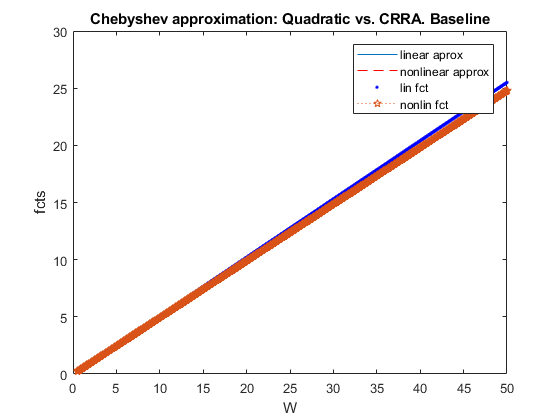
\includegraphics[width = .8\textwidth, keepaspectratio]{ps4ex2fig1.png}
\end{center}
\end{figure}

\begin{figure}[h!]\begin{center}
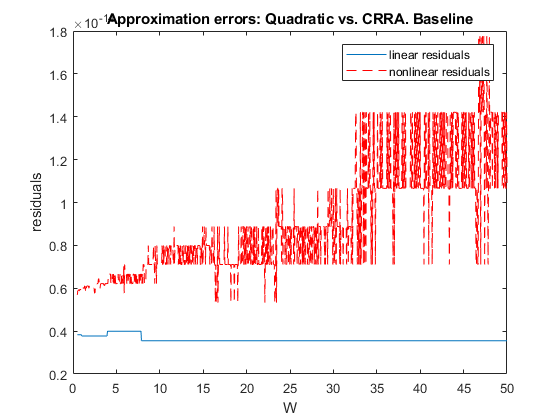
\includegraphics[width = .8\textwidth, keepaspectratio]{ps4ex2fig2.png}\end{center}
\end{figure}

\begin{table}[H]
\centering
\caption{Maximum percentage errors of deviation}
\vspace{.5cm}
\begin{tabular}{rlcc}
\hline
 & Setting & Example & MPE of deviation \\[.5em]
 \hline
 & Baseline & & 2.75 \\[1em]
 (i) & Higher risk aversion $\gamma$ & $\gamma = 4$ & 4.22 \\[1em]
 (ii) & Lower probability $p$ & $p = 0.20$ & 3.55 \\[1em]
 (iii) & Higher mean-preserving interest rate spread & +0.40 & 19.17\\[1em]
 \hline
\end{tabular}
\end{table}

The table shows that the maximum percentage error of deviation increases for all modifications (i)-(iii) compared to the baseline model. In particular, the error of deviation significantly increases if agents face higher spreads. However, it is naturally impossible to compare these change quantitatively since we plugged in some arbitrary numbers to mimic the new setting. Different values will produce different errors, but we can safely say that errors of deviation generally increase.

\section{Question 3}

\subsection{}	
Using $p:=p_l$ and therefore  $1-p=p_h$ the first order condition of agent $i$ becomes  \begin{align}\scriptstyle
\frac{1-\gamma_i}{1-\gamma_i} \left[p\, (1+r^f+\alpha(r_L-r^f))^{-\gamma_i}(r_L-r^f) +(1-p)\, (1+r^f+\alpha(r_H-r^f))^{-\gamma_i}(r_H-r^f)\right]&= 0 \\ \Leftrightarrow E\left[ (1+r^f+\alpha(r-r^f))^{-\gamma_i}(r-r^f)\right]&=0 
\end{align}

\subsection{Analytical Solution of $\alpha_i$}
The equation has then been converted into the form $\alpha ( \gamma_i )$, already using the presented calibration.
\begin{align*}
E\left[ (1+r^f+\alpha(r-r^f))^{-\gamma_i}(r-r^f)\right] &= \\
p_l \left[ (1+r^f+\alpha(r-r^f))^{-\gamma_i}(r-r^f)\right] + p_h \left[ (1+r^f+\alpha(r-r^f))^{-\gamma_i}(r-r^f)\right] &= 0\\
0.1 (1.02 +\alpha(-0.06))^{-\gamma_i}(-0.06) + 0.9 (1.02+\alpha(0.06))^{-\gamma_i}(0.06) &= 0
\end{align*}
which can now be rearranged
\begin{align*}
0.1 (1.02 +\alpha(-0.06))^{-\gamma_i}0.06&=  0.9  (1.02+\alpha(0.06))^{-\gamma_i}(0.06) \\
0.1 (1.02 +\alpha(-0.06))^{-\gamma_i}&=  0.9  (1.02+\alpha(0.06))^{-\gamma_i} \\
\left(\frac{0.1}{0.9}\right)^{\frac{-1}{\gamma_i}} \left(1.02 +\alpha(-0.06)\right)&= 1.02+\alpha(0.06)\\
9^{\frac{1}{\gamma_i}} \left(1.02 +\alpha(-0.06)\right)&= 1.02+\alpha(0.06)\\
9^{\frac{1}{\gamma_i}} 1.02 - 1.02 &= \alpha(0.06) - \alpha(-0.06)9^{\frac{1}{\gamma_i}}\\
\alpha &= \frac{9^{\frac{1}{\gamma_i}} 1.02 - 1.02 }{(0.06) + (0.06)9^{\frac{1}{\gamma_i}}}
\end{align*}
This equation has then been approximated using Chebyshev and Spline interpolation.
\subsubsection{Chebyshev}
To approximate the function to the highest accuracy possible, Chebyshev nodes had to be created. \\
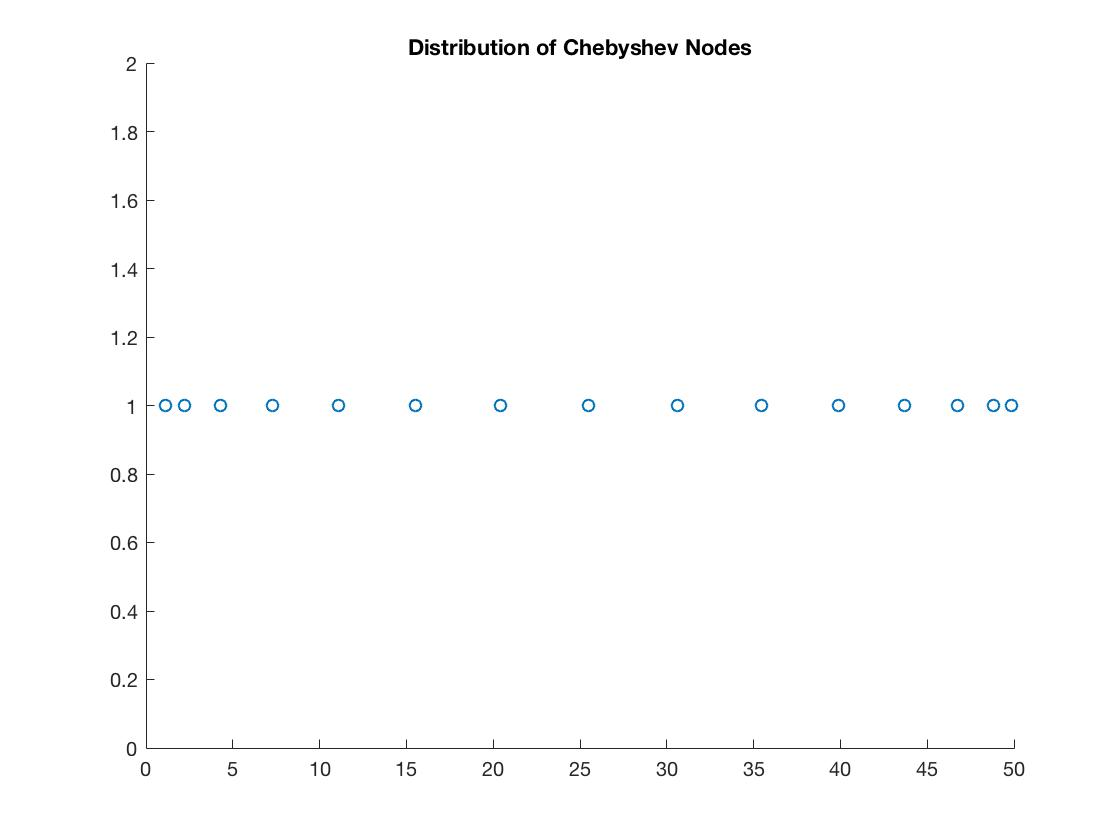
\includegraphics[width = \textwidth, keepaspectratio]{PS4Q3NODES.jpg} 
Then, the actual approximation could be performed. First, the unconstrained $\alpha$ has been approximated. \\
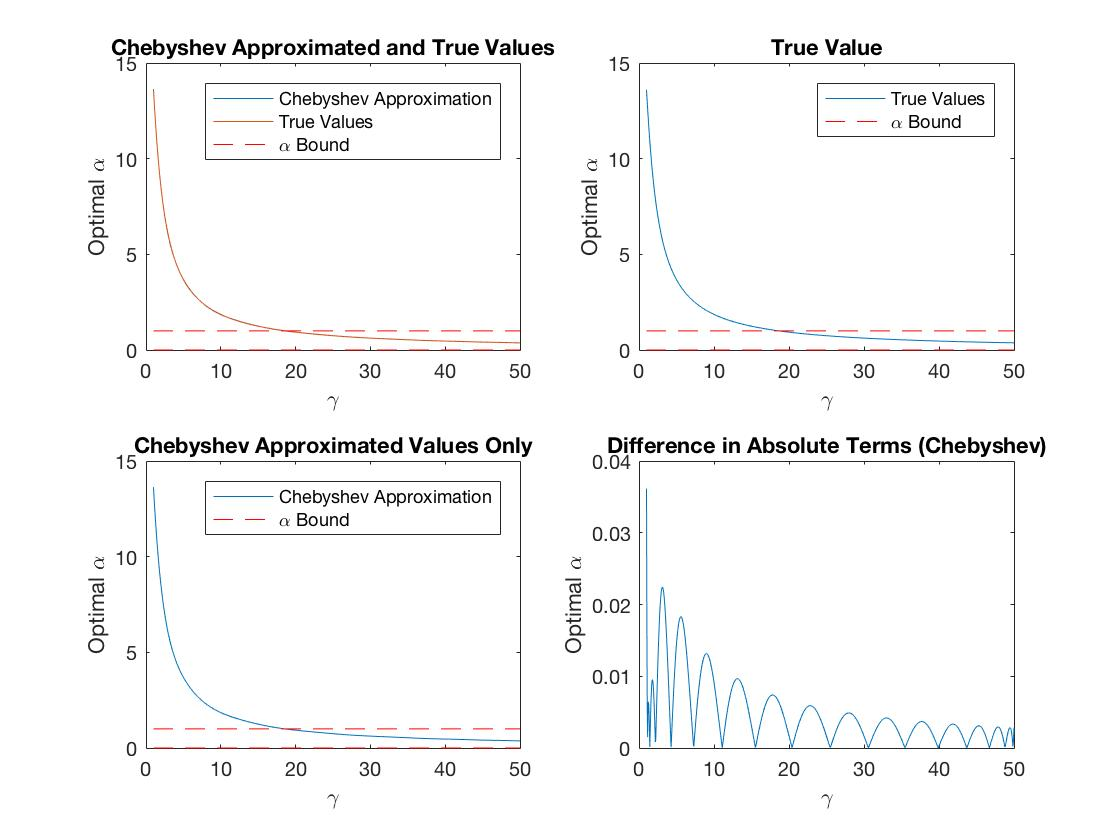
\includegraphics[width = \textwidth, keepaspectratio]{PS4Q3CHEB.jpg}
For the constrained $\alpha \in [0,1]$, we get:\\
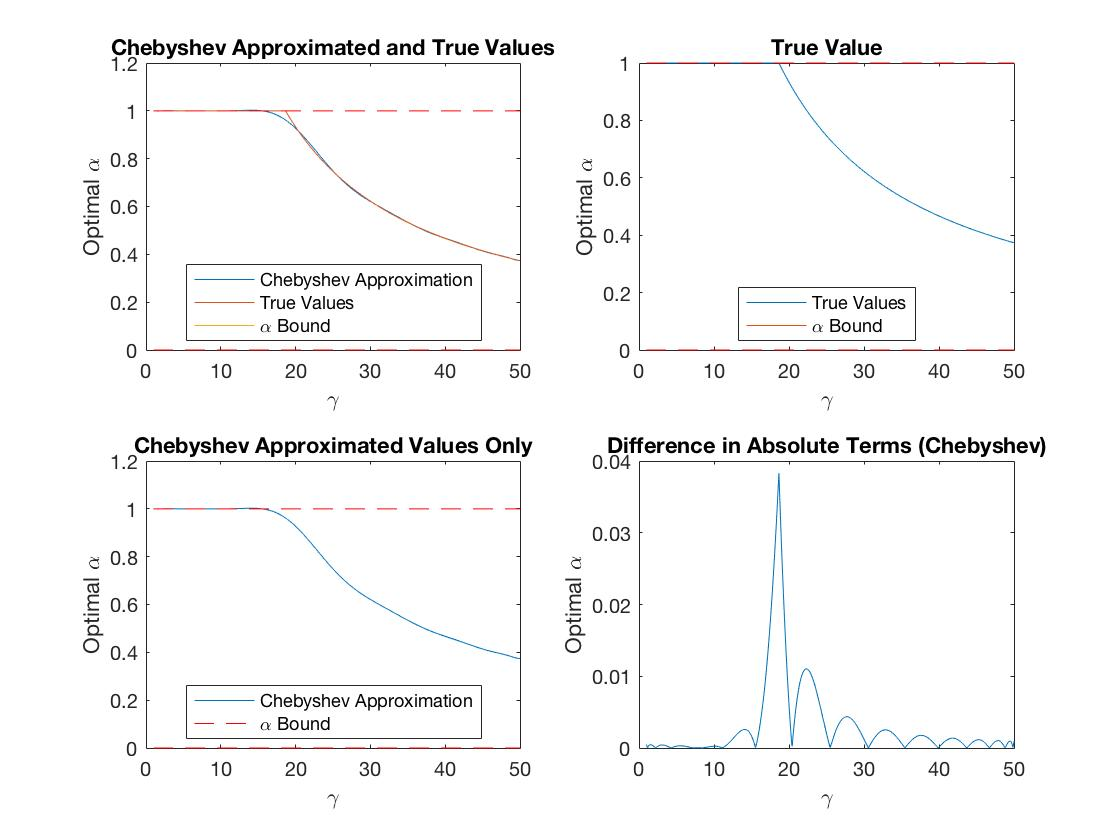
\includegraphics[width = \textwidth, keepaspectratio]{PS4Q3CHEB_constrained.jpg}
One can clearly see the spike in inaccuracy around the kink in the true function. 
\subsubsection{Spline Interpolation}
The Spline Interpolation has been performed by simply using the code provided as solution for the first exercise of this Problem set. Again, the interpolation is first performed on the unconstrained $\alpha$ and on the constrained one thereafter. \\
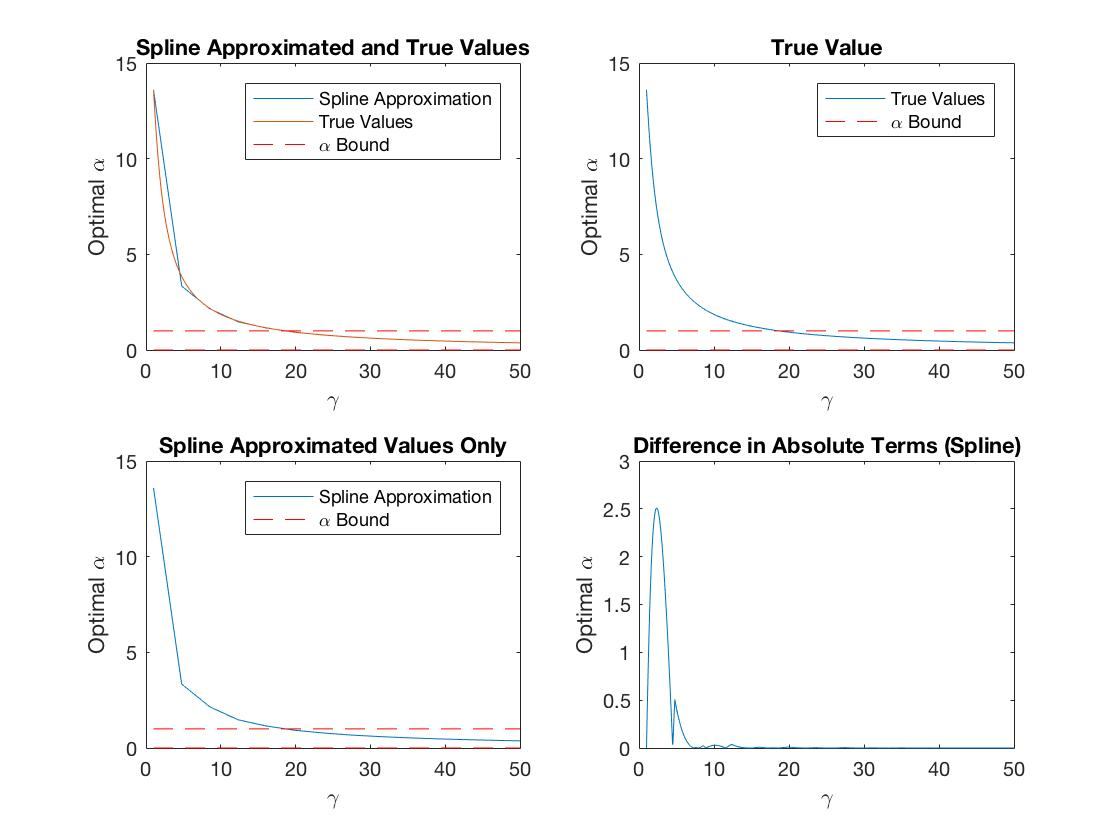
\includegraphics[width = \textwidth, keepaspectratio]{PS4Q3SPLINE.jpg} 
As before for the Chebyshev approximation, the approximation with linear splines for the constrained $\alpha$ differs:\\
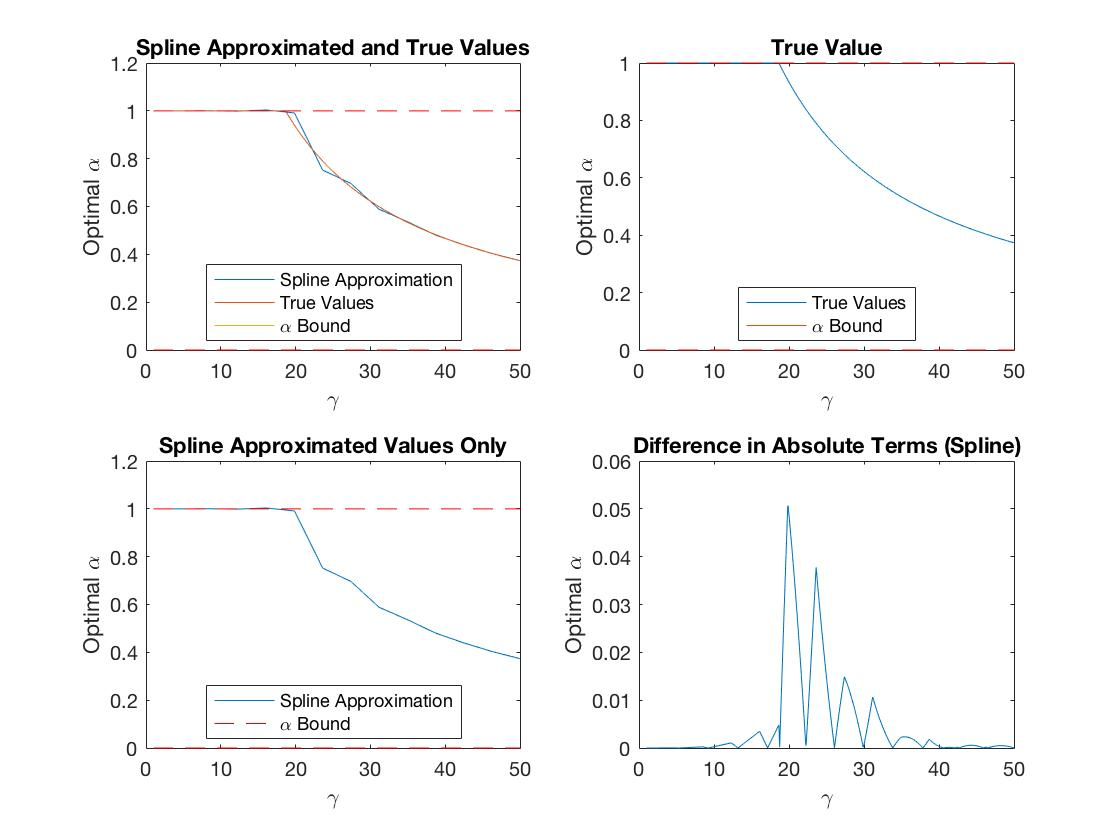
\includegraphics[width = \textwidth, keepaspectratio]{PS4Q3SPLINE_constrained.jpg}
Again, the error increases around the point of the kink. The quality of this approximation technique could be increased by adaptive grid methods, adding nodes where the difference between the approximation is the largest (i.e. right at the point of the kink).
This has been tried out but did not fully work out as planned. However, an improvement can be seen from using an adjusted grid:\\
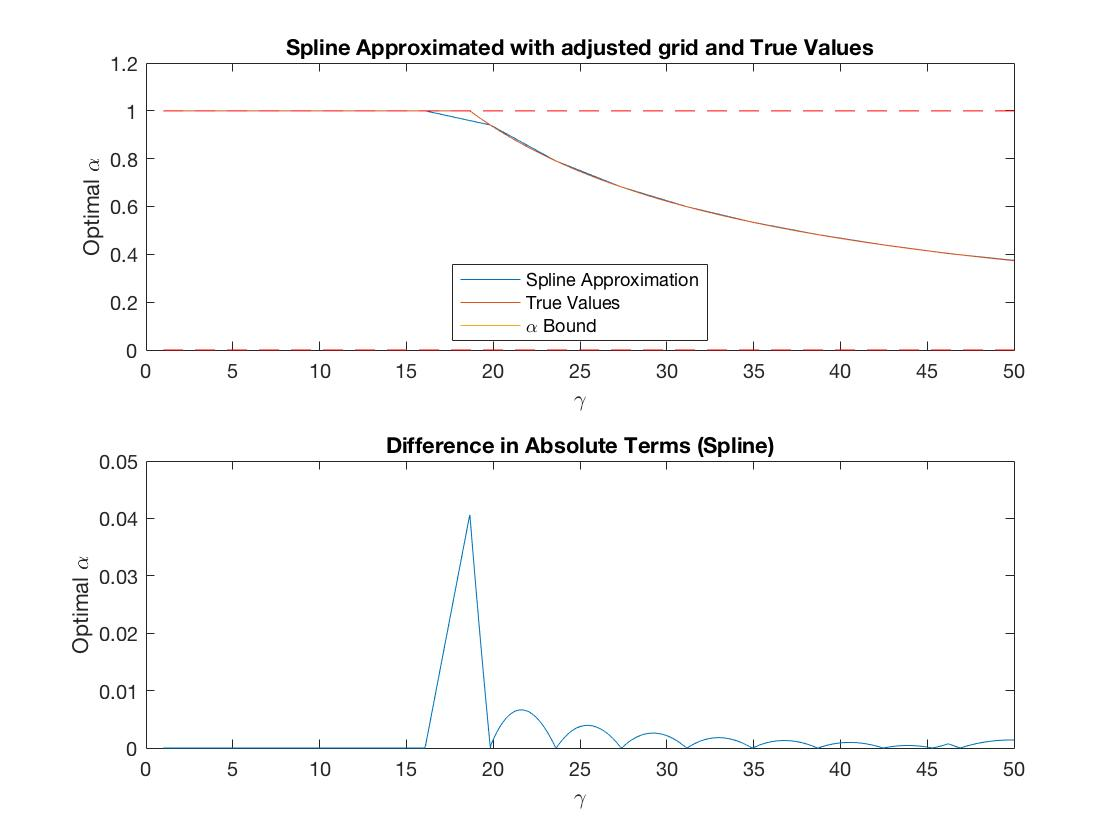
\includegraphics[width = \textwidth, keepaspectratio]{PS4Q3SPLINE_constrained_adjusted.jpg}
\subsection{Analytical Solution of $\gamma_i$}
The formula stated on the exercise sheet  displays that the first derivate of the objective function with respect to $\alpha_i$ evaluated at $\alpha_i=1$ has to be equal zero. That is, agent $i$'s optimal portfolio share is one or in other words, the constraint imposed just binds from above. Indeed, this expression can be rewritten in terms of its associated degree of risk aversion: \begin{align*}
\gamma_i^*=\frac{\ln{1-p}-\ln{p}}{\ln {1+r_H}-\ln {1+r_L}}
\end{align*}
\newpage
\begin{appendices}
\section{Code to Question 1}
Chebyshev Approximation:
\lstinputlisting[style=Matlab-editor]{cheb.m}
Linear and cubic splines, also using the Miranda-Fackler toolbox:
\lstinputlisting[style=Matlab-editor]{spl.m}
Function to be approximated:
\lstinputlisting[style=Matlab-editor]{simplef.m}
Main code:
\lstinputlisting[style=Matlab-editor]{PS4P1.m}
\section{Code to Question 2}
\lstinputlisting[style=Matlab-editor]{ps4ex2_new.m}
\section{Code to Question 3}
Main code:
\lstinputlisting[style=Matlab-editor]{main.m}
The function to be approximated:
\lstinputlisting[style=Matlab-editor]{simplefQ4P3.m}
With constraint:
\lstinputlisting[style=Matlab-editor]{simplefQ4P3const.m}
Chebyshev:
\lstinputlisting[style=Matlab-editor]{chebi.m}
Spline:
\lstinputlisting[style=Matlab-editor]{spl.m}
\end{appendices}

\end{document}